\section{A.2 Welleneigenschaften von Teilchen}

Teilchen weisen auch Welleneigenschaften auf
\\
\\
es gilt: \mbox{\Large $\lambda_{Br} = \frac{h}{p} = \frac{h}{m \cdot v}$}
\\
\\
Elektron mit \mbox{\Large $ v = 100 \frac{km}{s} \,\to\, \lambda_{Br} = 1,4 \cdot 10^{-12}m$}
\\
\\
Nachweis:
{\color{red}
\begin{itemize}
    \item Deutliche Beugungserscheinungen treten auf, sofern $\lambda \approx$ Spaltbreite ist
    \item Kristallgitter weisen entsprechende Abstände auf
    \item $ \Rightarrow$ Beugung von Elektronen an Kristallgitter $\,\to\,$ es treten Beugungsfiguren auf
\end{itemize}
}
\subsection{Doppelspaltesperiment}

Siehe \url{https://tinyurl.com/yhyekk7x}
\\
\\
Ein Teilchen kann sich nicht nur einmal als Teilchen und einmal als Welle verhalten, sondern noch dazu konform zur Erwartungshaltung des Beobachters.
\\
\\
Es gibt einen fundermentalen Unterschied zwischen Welle und Teilchen.
\\
\\
{ \color{red} Ein Teilchen ist lokalisierbar}
\\
\\
Überlagerung einer großen Zahl unendlicher Wellen mit leicht unterschiedlichen Wellenlängen ergibt eine Wellengruppe, die sicht mit $v$
vorwärtsbewegt (Realisierung der Lokalisierbarkeit eines Teilchens). Realisieren, dass Aufenhaltsort mit der Zeit immer ungenauer wird
($\,\to\,$ Zerfließen des Wellenpaketes).
\\
\\
Aufenhaltswahrscheinlichkeit \mbox{\Large $ \{Psi = (Amplitude\,A)^2$}
\\
\\
Die Wahrscheinlichkeit, dass Teilchen an einem bestimmten Ort zu finden.
\newpage
1. Fall: Teilchen in einem unendlichen Potentialkasten
    \begin{figure}[h]
        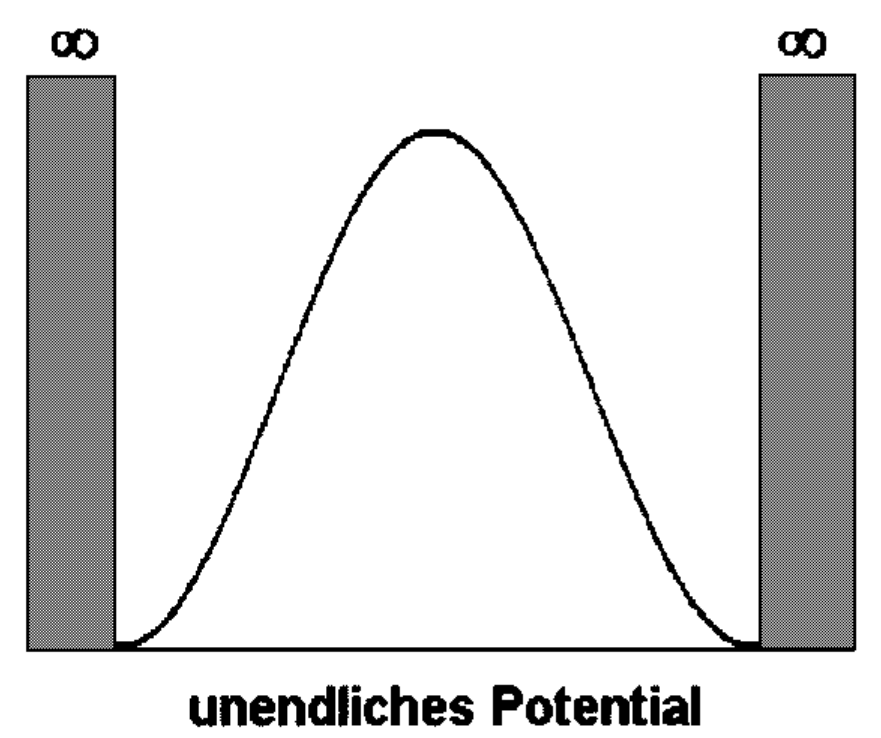
\includegraphics[width=0.4\textwidth]{media/unendlichesPotential.png}
        \label{fig:meine-grafik}
    \end{figure}
\\
\\
im Potentialkasten \mbox{\Large $\Psi > 0$}
\\
außerhalb \mbox{\Large $\Psi = 0$}
\\
\\
2. Fall: Teilchen im endlichen Potentialkasten
\\
    \begin{figure}[h]
        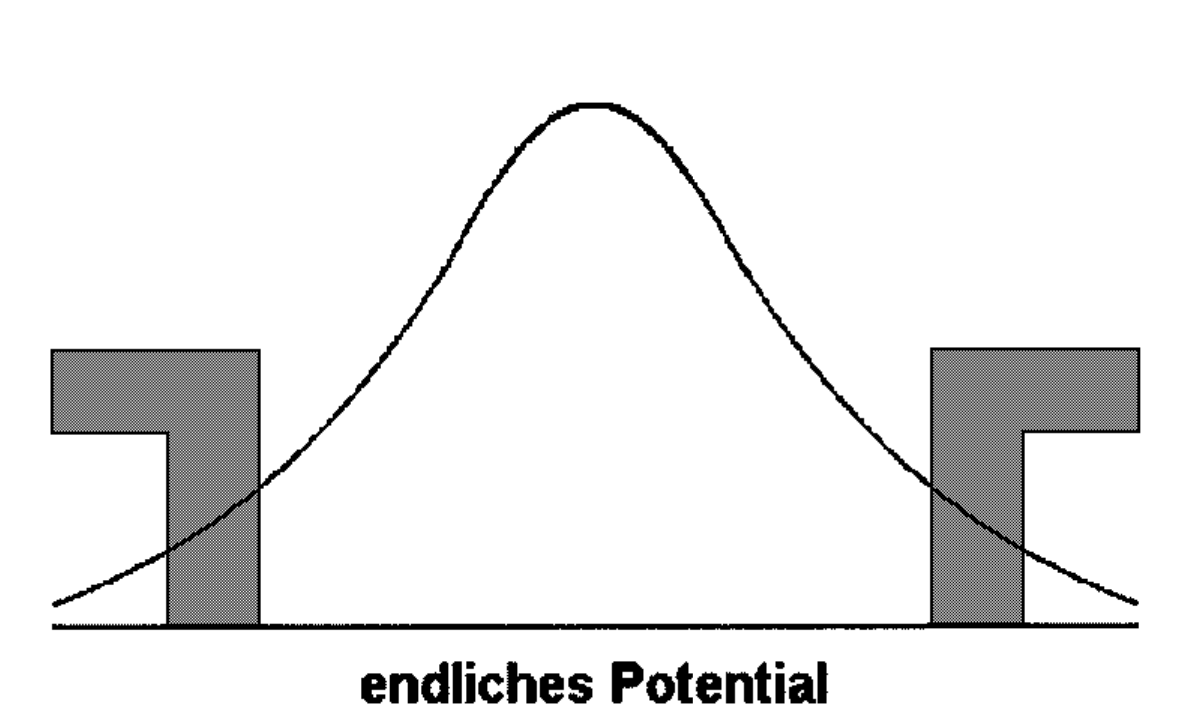
\includegraphics[width=0.4\textwidth]{media/endlichesPotential.png}
        \label{fig:meine-grafik}
    \end{figure}
\\
\mbox{\Large $\Psi > 0$} an den Rändern
\\
\mbox{\Large $\Psi > 0$} außerhalb des Potentialkastens
\\
$\Rightarrow$ Tunneleffekt
\\
\\
Tunneleffekt spielt nur im Mikrokosmos eine Rolle
\\
\\
Beispiel: $\alpha$-Zerfall (He-Kerne, die von angeregten Kernen emittiert werden)
\\
$\alpha$-Teilchen tunnelt durch Kernpotential ($\alpha$-Teilchen als Welle in endlichen 
Potential) $\,\to\,$ Aufenhaltswahrscheinlichkeit $\,\to\,$ mittlere Zeit, dass das Teilchen
a außerhalb des Kerns zu finden $\Rightarrow$ Halbwertszeit
